%\documentclass[a4paper,11pt]{report}
\documentclass[onecolumn,traditabstract]{aa}
\usepackage[pdftex]{graphicx}
\usepackage{natbib}
\usepackage{txfonts}
\usepackage{blindtext}
%-------------------------------------------------------------------
\bibpunct{(}{)}{;}{a}{}{,} % to follow the A&A style
\bibliographystyle{aa} % style aa.bst
%-------------------------------------------------------------------
% Instrument (%sign  comment in or out)
%-------------------------------------------------------------------
%\blank

%-------------------------------------------------------------------
% Title (replace content)
%-------------------------------------------------------------------
\title{High resolution observations of the thermal SZ effect on galaxy clusters}
\author{{\bf Coordinators: }J.F. Mac�as-P�rez (LPSC), B. Comis (LPSC), E. Pointecouteau (IRAP),Team: R. Adam (LPSC), N. Aghanim (IAS), M. Arnaud (CEA), F.X. Desert (IPAG), M. Douspis (IAS), F. Mayet (LPSC), P. Mauskopf, J.B. Melin (CEA), L. Perotto, G. Pratt (CEA)}
%\date{September 1994}
\begin{document}
\maketitle
%\clearpage

\abstract{We describe here the NIKA2 Guaranteed Time Large Program dedicated to high resolution observations of clusters of galaxies at intermediate and high redshift via the thermal Sunyaev-Zeldovich (tSZ) effect for a total of 300 hours. NIKA2 is well adapted for high angular resolution follow-up observations of an SZ selected cluster sample because of its large number of high sensitive detectors at two frequency bands (150 and 260 GHz), its large field of view (6.5 arcmin) and the resolution allowed by a 30 m telescope (17.5 and 11 arcsec for the NIKA2 frequencies). We intend to observe a large ($\gtrsim$ 50) and cosmologically representative sample of clusters of galaxies, with redshift between 0.5 and 1.5, to which the f.o.v. and resolution of NIKA2 are better suited. The main output of the program will be the study of the redshift evolution of the cluster pressure profiles as well as of the scaling laws relating cluster observational parameters, Y (integrated Compton parameter), Y$_{X}$ (X-ray mass proxy), and T$_e$ (electron temperature) for example, to their total mass. This will be achieved by combining the NIKA2 data with ancillary data including X-rays and optical observations and will lead to significant improvements on the use of clusters of galaxies to draw cosmological constraints.} 


\section{Scientific context}
As the largest gravitationally collapsed objects, clusters of galaxies represent the last step of the hierarchical gravitational process of structure formation. Therefore their abundance and evolution are strictly related to the power spectrum of the primordial density fluctuations, cosmological parameters and their evolution all along the history of our Universe.
Clusters are mainly made up of dark matter (85\%), while most of the baryons are present as a diffuse gas, the Intra-Cluster Medium (ICM), hot (10$^6$ ? 10$^8$ K) and completely ionized because of the incredibly high masses characterizing this kind of structures (10$^{13}$ - 10$^{15}$ M$_{\odot}$). Since the ICM is a very good tracer of the dark matter distribution, ICM observables can provide a valuable tool for cosmological investigation with clusters, as long as we are able to convert them into mass estimates. From baryonic observables the total mass can be inferred through scaling relations, which corresponds to power laws obtained in a simplified scenario in which gravity is the only process driving cluster evolution. At present, the systematic uncertainties affecting the observable to mass relations represent the limit for cluster-derived cosmological constraints.
Due to its physical state, the ICM is responsible of a secondary anisotropy of the Cosmic Microwave Background (CMB), which is the thermal Sunyaev-Zel?dovich (SZ) effect. Through their path toward us, CMB photons interact with free hot electrons in the ICM. After this interaction a fraction of CMB photons is moved to higher energies, with a resulting flux decrement (increment) at frequencies below (above) 217 GHz. The amplitude of the deformation is proportional to the integral of the pressure of the electron population along the line of sight. While optical and X-ray cluster signals are affected by cosmological dimming, this is not the case for the tSZ cluster signal. Therefore the tSZ effect allows us to detect and study cluster of galaxies at high redshifts, where their number and distribution is the most sensitive to the underlying cosmology.
In the last few years, tSZ-selected cluster catalogues containing hundreds of candidates have finally been produced, with arcmin resolution, by the South Pole Telescope SPT \citep{Reichardt2013, Bleem2014}, the Atacama Cosmology Telescope (ACT, Hasselfield \& ACT Collaboration 2013), the Planck Satellite \citep{PSZ1, PSZ2}. The use of tSZ- selected cluster samples for cosmological purposes requires the understanding of how matter is distributed and the evaluation of the scatter that disturbed systems may introduce in the tSZ integrate flux (Y) to total cluster mass (M) relation. The Planck, ACT, SPT resolutions ($\gtrsim$ 1 arcmin) only allow detailed study of spatial distribution of low redshift clusters (z $<$ 0.2). Therefore, sub-arcminute angular resolution measurements of cluster pressure profiles are a mandatory step for precise cluster cosmology. Moreover, pressure profiles ? P$_e$(r) ? with spatial resolution comparable to those of X-ray derived electron densities ? n$_e$(r) ? can also be used to study the cluster radial distribution of temperature ? T$_{e}$(r) $\propto$ P$_{e}$(r)/n$_{e}$(r) ? and entropy (K(r) $\propto$ P$_{e}$(r)n$_{e}^{-5/3}$), which are essential to unveil cluster thermodynamic history.
\paragraph{{\large Context} --}
Technological progress have made the tSZ effect routinely detected, and we are now just starting to exploit this extremely powerful tool to investigate the physics of the cluster population up to large redshifts ($z$). In fact, since the observable is not the cluster itself but the spectral distortion of the CMB, the tSZ effect could provide a redshift independent probe of the pressure of the electron population that produced it. It is therefore an alternative tool to {\bf investigate less dense regions} of the clusters and their evolution {\bf up to large $z$}, as long as an adequate angular resolution is reachable.
In the last few years, tSZ-selected cluster catalogues containing hundreds of candidates (with arcmin resolution) have finally been produced by the South Pole Telescope \citep[SPT, ][]{Reichardt2013, Bleem2014}, the Atacama Cosmology Telescope \citep[ACT, ][]{Hasselfield, Hasselfield2013} and  the Planck Satellite \citep{PSZ1}. The Planck satellite has already detected many clusters through tSZ, performing a blind survey able to use this effect to identify objects not yet discovered at other wavelengths \citep{PSZ1}. Because of the poor resolution of the Planck satellite (5 arcmin), high-resolution complementary observations and follow-ups are now necessary to explore the cluster internal structure more deeply. The NIKA camera at the IRAM 30~m telescope is a well-suited instrument for such observations and follow-ups, given its resolution, sensitivity and dual-band observation capability (as it will be detailed later).

\paragraph{Past or ongoing programs and concurrent instruments}
Interferometer (i.e. AMI, AMiBA, CARMA, ALMA) can reach extremely high angular resolutions, but they cannot recover the large scale signal and they are time expensive. Other experiences operate at the focus of large diameter telescopes (Mustang and Mustang2 at GBT, Bolocam and BolocamII at LMT). But none of them can combine a sufficiently large f.o.v. with the high angular resolution to explore the 0.1r$_{500}$ -r$_{500}$ radial range, and to that while observing simultaneously at two wavelengths. 
However the number of experiences able to 

\paragraph{Main scientific goals}
Clusters grow by constant smooth accretion and violent merger events. This mechanism driving
the growth of structures impacts cluster content, and thereby this complex accretion history imprint
ICM which is known to counter balance the gravitational radiative cooling of the hot gas. This
the physical state and properties of the hot intra-cluster gas. Furthermore feedback from galaxy formation (through AGN and SFR/SN) impacts the properties of the gas. It injects energy within the
energy injection also modifies the thermodynamical state of the ICM.
We have now a fairly good view of properties for the hot ICM gas in the local Universe, mainly
redshift below 0.5. This has been possible because of recent tSZ measurements that are a
powerful diagnostic of the ICM physical state. Indeed the tSZ effect is directly proportional to the
thermal pressure integrated along the line of sight. Measuring the (radial) distribution of the SZ
signal in clusters directly provide this of the thermal pressure of the ICM. By contrast X-ray
measurements are sensitive to the square of the gas density and the root square of the
temperature. We present in Figure 1 recent measurements of the stacked cluster radial pressure 
profile using tSZ observations with PLANCK, BOLOCAM and SPT and X-ray estimates. From the
left plot we can notice that the tSZ measurements are in good agreement but are not able to
sample the inner part of the clusters, which present a cool-core (CC), and disturbed ones (non-CC). This is more obvious 
...
In addition, we still need to investigate how cluster properties evolve with time in order to understand the mechanisms ruling the formation and the evolution of structure.
The investigation of the physical state of group and clusters with redshift will thus help us to asses 
the evolution involved by the cluster accretion history, the process of in a gravitationally bound
system and by the co-evolution between the baryonic component of clusters, i.e., the hot intra-
cluster gas and the cluster galaxies. Carrying such a study over a population of high redshift
clusters will allow to quantify whether the thermal content and its distribution evolve as massive
halos continue to growth through accretion and merger. Such measurement will be only possible thanks to the high sensitivity and high spatial resolution tSZ observations. As discussed below NIKA2 is an ideal instrument to carry such observations.

Furthermore, the natural combination of direct observables of the intra-cluster hot gas (i.e., SZ and X-ray measurements) as well as of the dark matter distribution (i.e, optical weak lensing measurements), will allow a full physical characterization of the (radial) distribution of the physical properties of clusters including pressure, entropy, gas mass, total mass, gas fraction and clumpiness of the gas. Indeed, the tSZ signal directly provides the gas pressure, where the X-ray data delivers the gas density squared and temperature. The combination of the two observables is the only way to provided an unbiased estimate of the entropy and clumpiness of the gas. In addition, weak lensing measurements will provide complementary measurements of the dark matter distribution and total mass of the cluster with totally independent systematics.

Global quantities will derived from 1D (radial profiles) and 2D (maps) analysis in to order to provide further constraints on the evolution of clusters scaling relations (Y-Yx, M-Y, S-Y, etc). Furthermore, the combination of the SZ and X-ray data to optical/NIR observations of the cluster galaxies will further help to investigate the connection between galaxy properties (luminosity function, SFR, stellar mass) and these of the ICM, and thereby bring constraints on feedback mechanisms at play within clusters.

These in depth investigations over a large redshift range will bring detailed insight of the properties of clusters over more than 3 Gyr, allowing us to understand the processes driving the physical evolution of massive halos in the universe.

\paragraph{NIKA2 specifics for SZ observations}
\begin{figure}
  \begin{center}
   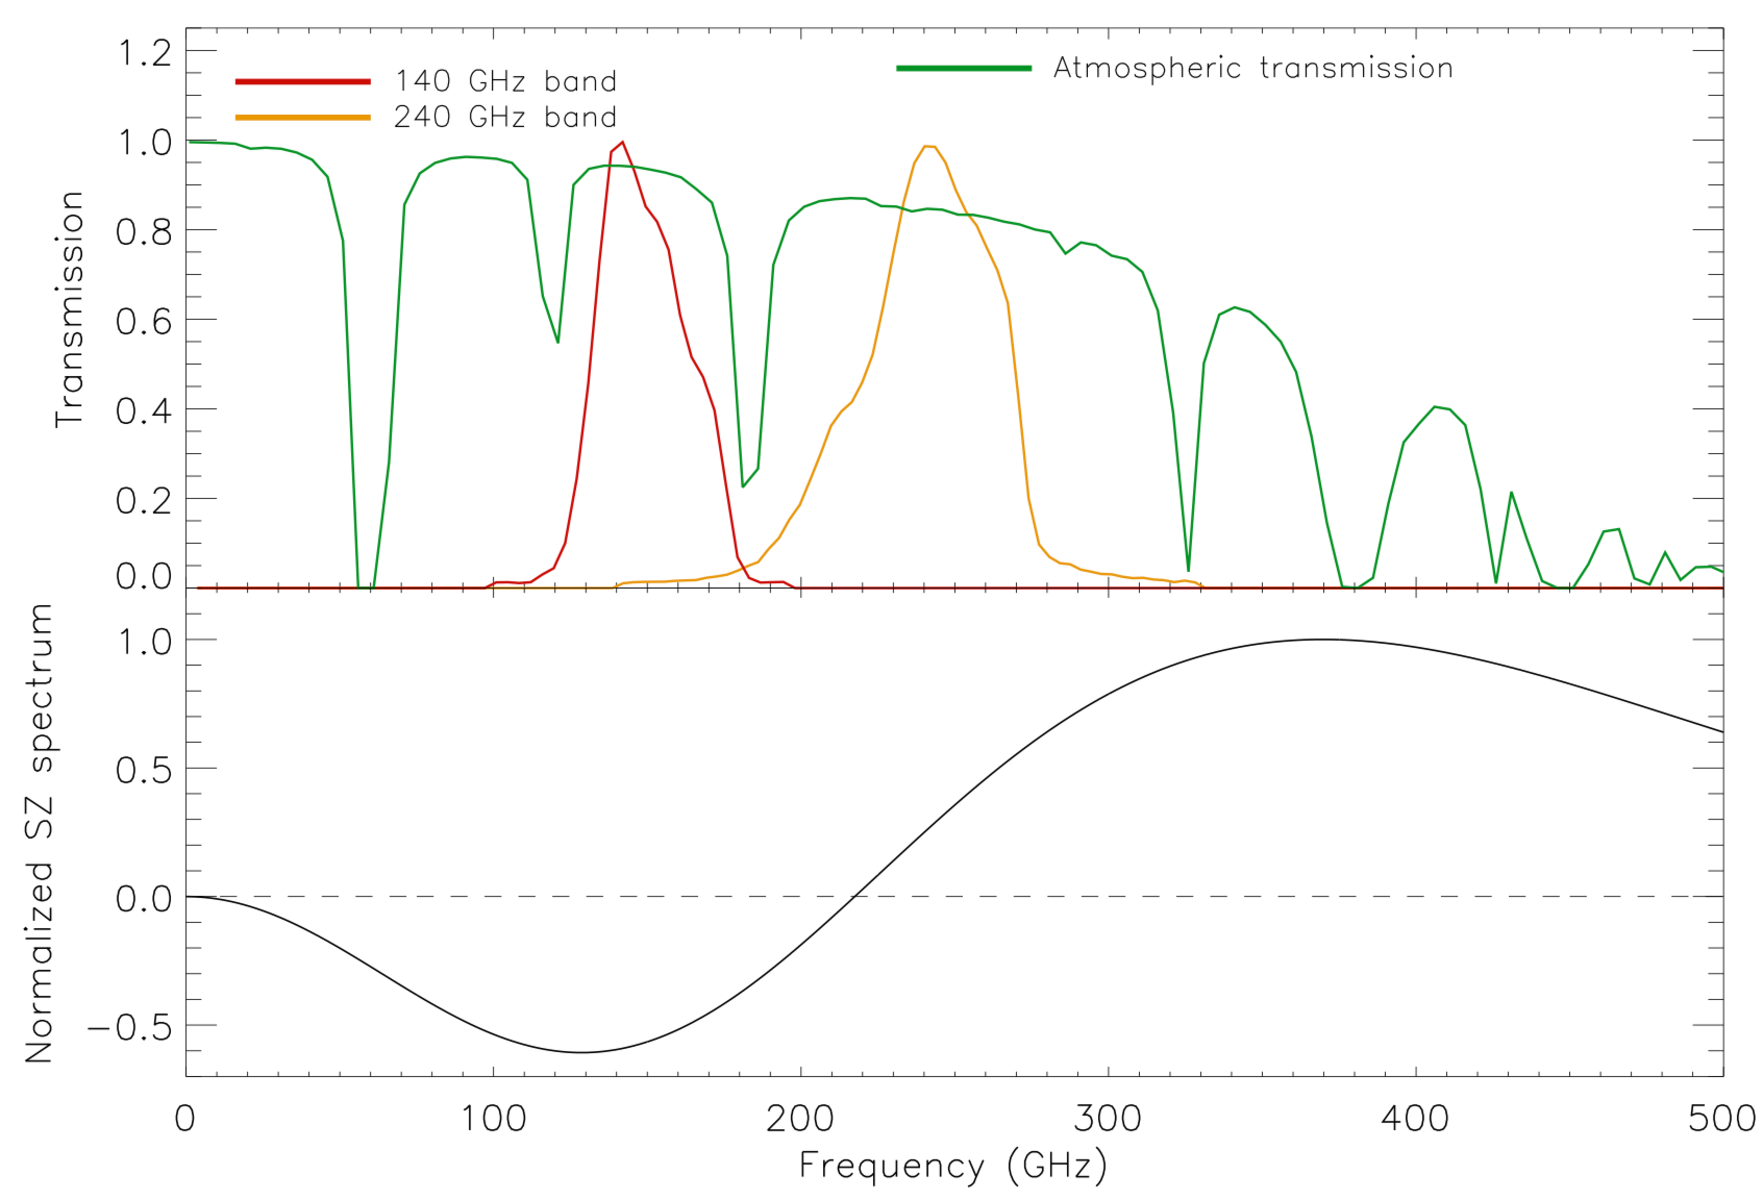
\includegraphics[width=0.6\columnwidth]{./Figures/NIKA_bp_sz.pdf}
  \end{center}
\caption{{\bf Top:} The bandpasses of the current NIKA KIDs arrays at 140 (red) and 240 (orange) GHz and the atmospheric transmission at Pico Veleta (Spain), the IRAM 30m telescope site. {\bf Bottom} The spectral distortion of the CMB intensity induced by the tSZ effect.}
\label{Fig:bands}
\end{figure}

The NIKA2 camera is particularly well adapted for high resolution observations of the tSZ effect on cluster of galaxies:
a) it operates simultaneously at two frequency bands: 150 and 260 GHz. As shown on the bottom panel of Figure \ref{Fig:bands} we expect for 150 and 260 GHz a negative and a positive distortion of the CMB spectrum producing a very distinctive cluster signal on the observed maps. The latter is demonstrated on the right panel of the figure where we present Planck satellite observations of a cluster of galaxies at 143, 217 and 353 GHz.
b) NIKA2 is made of arrays of thousands of high sensitive Kinetic Inductance Detectors (KIDs). In particular we expect a sensitivity in Compton parameter units of 1.13 x10$^{-4}$ per hour and per beam. This should allow us to obtain reliable tSZ detections of clusters of galaxies in few hours.
c) NIKA2 coupled to the IRAM 30 m telescope should allows us to map clusters of galaxies to a resolution of typically 12 to 20 arcsec within a 6.5 arcmin diameter FOV. This is well adapted for medium and high redshift clusters for which we expect typical angular sizes of about 6-11 arcmin as shown on the left panel of Figure 3.

The interest of NIKA2 for tSZ observations of clusters of galaxies has already been partially demonstrated by the results of NIKA, which is a prototype instrument operated at the IRAM 30 m telescope with two frequency bands (140 and 240) and 300 KIDs in total. This is shown on the right panel of Figure 3 where we present a 140 GHz tSZ map of the RXJ1347.5-1145 cluster.
It is important to compare the NIKA2 instrument to other existing and planned instruments for high resolution tSZ observations. For this purpose we list below the main characteristics for the most relevant ones:
- BOLOCAM: 144 bolometer arrays operated at the 10 m CSO telescope at 140 and 268 GHz, with
58 and 31 arcsec resolution, over a 8 arcmin diameter FOV.
- MUSTANG/GBT: 64 element bolometer array operating at 90 GHz on the 100 m GBT telescope
with a resolution of 8.5 arcsec
- CARMA: 23-element multi-frequency interferometer at 31, 86 and 90 GHz

\paragraph{Target selection}
The main objective of this program is to obtain high resolution tSZ observations of a cosmological representative sample of clusters of galaxies at intermediate and high redshifts, z > 0.5, to study the evolution of cluster physical properties across cosmic times.
The selection is then mainly driven by the need of an homogeneous coverage in SZ flux. A flux selected subset of the cluster population is then representative of a sample that is not biased towrds a given morphology (+ selection function). 
In order to fulfill this objective given the limited total observing time, 300 hours, we consider the following target selection criteria:
- clusters belonging to SZ selected samples
- clusters from already existing tSZ based cluster samples and in particular from the Planck, ACT and APEX-SZ samples for which we already have estimates of the total tSZ flux (see Figure 4 for details)
- limit sample to clusters in the redshift range from 0.5 to 1.5
- reliable tSZ mapping for each cluster should not exceed 4 hours of on target observations so that the total number of observed cluster is larger than 50
- clusters observed in X-rays (by XMM or Chandra)
- clusters for which weak lensing information is available - include backup objects

Because we want to derive relation that can be applicable to the whole cluster population (not only relaxed or un-relaxed). Study the relations, the source of the scatter the statistics of the morphology.
We aim for a good global characterization of the cluster population.

{\bf Preliminary list of targets}
The current status of the follow-up observations discussed above (not fully finished) does not allow us to present a definitive catalogue of clusters of galaxies. However, using the above criteria and the Planck and ACT samples we have pre-selected a first sample of clusters of galaxies suitable for our purposes. Notice that for the ACT clusters we do not dispose yet of redshift and we have selected all of them for simplicity. For the CLASH sample, well known disturbed clusters are removed. Furthermore, we consider only clusters that visible with the IRAM 30 m telescopes. Figure 4 shows a mollwide representation of the pre-selected sample, which is detailed in Table 1.

	

\bibliography{biblio}



\end{document}
